%% The following is a directive for TeXShop to indicate the main file
%%!TEX root = diss.tex

\chapter{A new taxonomy of 3D Reconstruction}
\label{ch:3DRecon_Taxo}
Existing taxonomies of 3D reconstruction techniques generally only focus on one category of techniques: ~\citeauthor{seitz2006comparison} proposed  multiple means to classify Multi-view Stereo algorithms from various perspectives. Reviews \cite{geng2011structured, salvi2004pattern} of Structured Light techniques generally classify techniques based on the type of pattern used. Photometric Stereo algorithms are classified by the assumptions or generalizations made, for instance, calibrated/uncalibrated, unknown/known reflectance, unknown/known light conditions, etc. This framework provides a means to compare intra-category algorithms, but is unsuitable to evaluate the performance of each technique across object with a range of attributes.

To have a more comprehensive understanding of the strengths and weaknesses of different techniques, a more general taxonomy is need, and one of the most popular framework categorizes 3D reconstruction techniques into active and passive methods: if the controlled light condition is used, then it's active, otherwise, it's passive. Other notable taxonomy is the spacetime framework proposed in \cite{davis2003spacetime}, which categorizes depth from triangulation techniques based on the sources of information: temporal or spatial information. Though widely adopted, the mapping of the algorithm to the conditions that works the best is generally empirical.

In the previous taxonomies, algorithms of a certain category generally work well on limited conditions, and a it's crucial to understand where algorithms perform well and where they fail. Under the previous framework, this knowledge is largely empirical, with each algorithm roughly maps to a problem domain that is poorly defined. 

The taxonomy proposed in this chapter defines the 3D reconstruction techniques based on the visual and geometric cues that techniques utilizes for reconstruction. This taxonomy transforms the 3D reconstruction problem from one requiring knowledge and expertise of specific algorithms in terms of how and when to use them, to one requiring knowledge of the visual and geometric properties of the target object.

3D reconstruction problem is classified into the following categories: stereo correspondence, shading, silhouette, texture, defocus.

We need to way general/univeral enough that incorporates any between-class methods, and distinctive enough that distinguish with-class methods. Thus we categorize our algorithms based on the \textit{setup}, \textit{information domain}, \textit{cue}, \textit{characteristics}, and \textit{representation}.

\section{Setup}
We consider setup using off-the-shelf hardwares, including camera, light sources, and projectors. Therefore commercial products such as laser scanner is not included.

Camera is the most basic component in any setup for reconstruction.

Light source is needed for any photometric stereo algorithms, the types of light sources include, but not limited to point light source, distant/directional light, and embient light.

\textbf{Point light} typically models nearby light source

\textbf{Directional light} assumes that all points in space share the same lighting direction which is only true when the light source is far away from the scene.

\textbf{Ambient light} model allows PS to work in less constrained lighting conditions. Ambient lighting could be considered as a spherical function.

For some methods, there is a need to project certain patterns onto the scene to help find correspondence. Therefore a projector is needed.

The typically setup for is shown in Figure~\ref{setup}.
\begin{figure}[h]
\centering
\begin{tabular}{ccc}
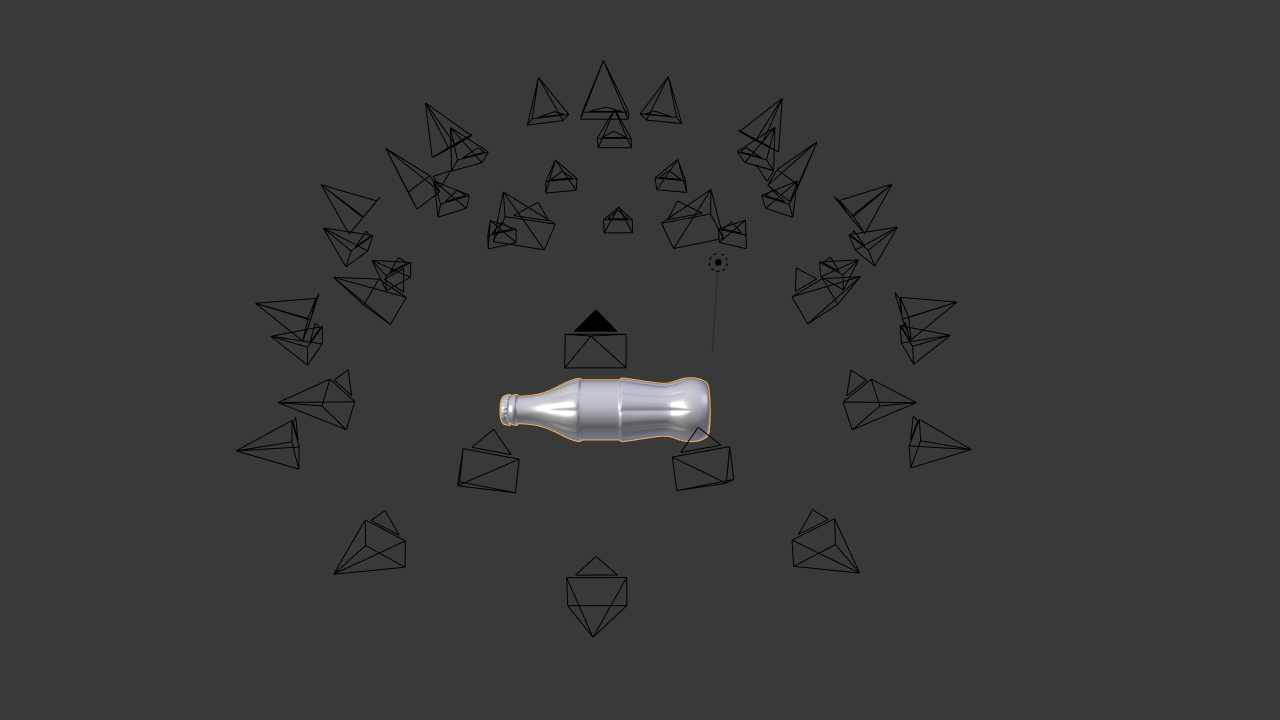
\includegraphics[width=0.33\textwidth]{taxo/mvs_setup}&
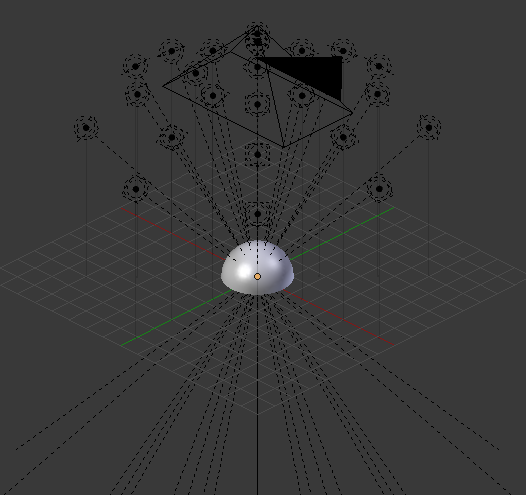
\includegraphics[width=0.33\textwidth]{taxo/ps_setup}&
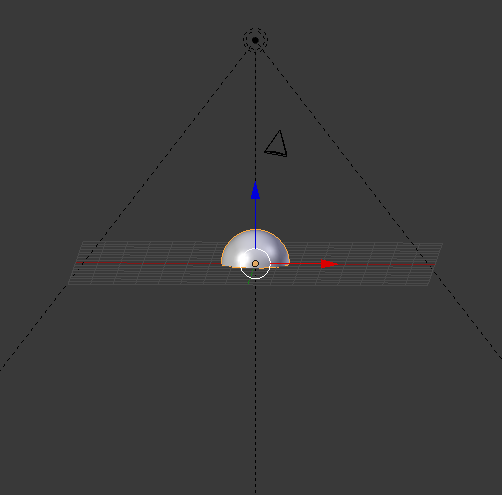
\includegraphics[width=0.33\textwidth]{taxo/sl_setup}\\
(MVS) & (PS) & (SL)\\
\end{tabular}
\caption{Typical setup of MVS, PS, and SL}
\label{fig:setup}
\end{figure}

\section{Information domain}
The information that is utilized for reconstruction can come from different domains. Techniques such as laser scanner and passive stereo typically utilize spatial information whereas methods such as structured light and temporal laser scanner make use of information across time. This criterion can bring together techniques that are considered separately by traditional active/passive taxonomy. We characterize the \textit{spacetime} domain in which the cues are located. The information can come from \textit{spatial domain}, or from \textit{temporal domain}. 
\begin{figure}[h]
\centering
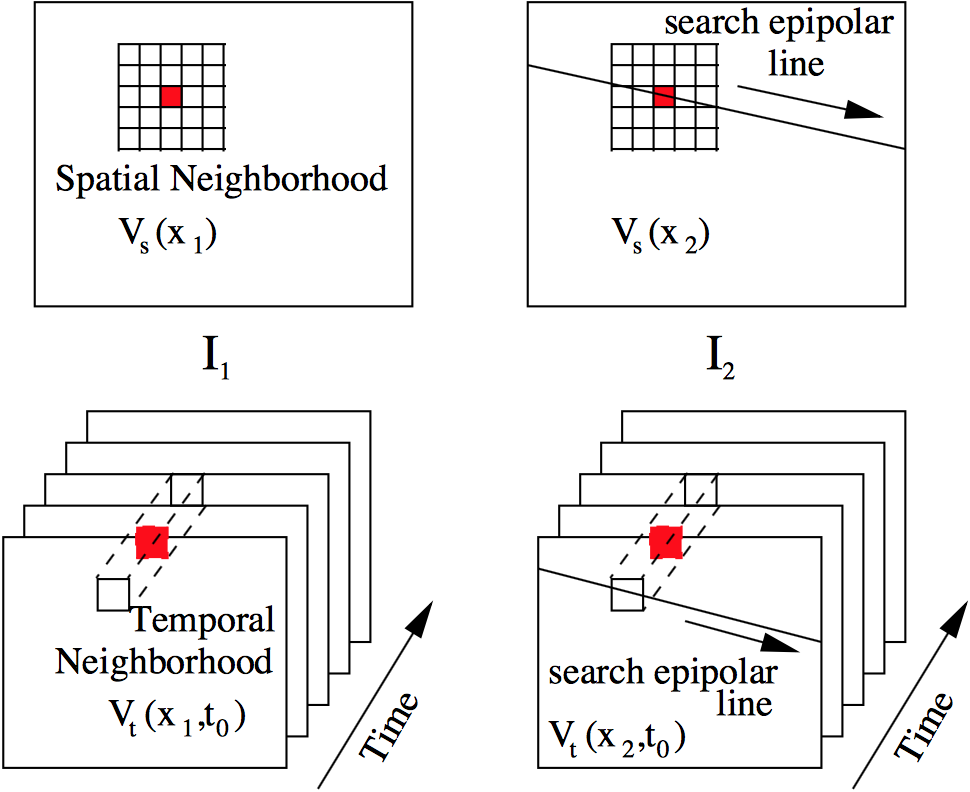
\includegraphics[width=0.8\textwidth]{taxo/spacetime_stereo}
\caption{Comparison of spatial (top) and temporal (bottom) stereo. In spatial stereo, the epipolar line is searched for similar spatial neighbourhoods. In temporal stereo, teh search is for similar temporal variation.}
\label{fig:spacetime_stereo}
\end{figure}

\section{Cue}
We discussed different visual/geometric cues that can be used by reconstruction algorithms in Chapter~\ref{ch:RelatedWork}, we classify them based on the spacetime domain that they occupy.
\subsection{Spatial cue}
\textbf{Texture} is the mostly used as spatial cue.

\textbf{Silhouette} is used by shape from silhouette and some stereo algorithms as an complementary cue, and is regarded as a spatial cue.

\subsection{Temporal cue}
\textbf{Intensity} variation of one pixel is used widely as the visual cue for photometric stereo. It is also the basis for temporal binary-encoded structured light techniques.

\section{Characteristics}
This is where we distinguish within-class methods.

\subsection{MVS}
As discussed in Chapter~\ref{ch:RelatedWork}, the MVS methods can generally be classified into four classes: 1). volumetric based methods compute a cost function in a 3D volume, and extracts a surface from this volume; 2). surface evolution based methods iteratively evolve a surface/volume to minimize a cost function; 3). seed propagation based methods start with a sparse set of scene points, and perform multiple iterations of propagations and refinements; and 4) depth-map based methods compute a per-view depth map and merge multiple depth maps into a complete 3D point cloud. We use the notation below to denote each class:
\begin{itemize}
\item Reconstruction algorithm: \textbf{V}: volumetric based methods; \textbf{E}: surface evolution based methods; \textbf{P}: seed propagation based methods; \textbf{D}: depth-map based methods.
\end{itemize}

\subsection{SL}
Structured light system overcomes the correspondence problem faced by any stereo technique by projecting a coded pattern onto the surface. The patterns are specifically designed so that codewords are assigned to a set of pixels, thus there is a direct mapping from the codewords to the coordinates of the corresponding pixel in the pattern. Based on the type of codeword used, the projection patterns are generally classified as: temporal encoding, spatial encoding, and direct encoding, refer to \cite{salvi2004pattern} for more details.

For temporal encoding, a set of patterns are successively projected onto the surface. The codeword is formed by a sequence of illumination for a specific pixel across the projected patterns. In the case of spatial encoding, the codeword of a point is obtained by considering the neighbourhood of the points around it. In the case of direct encoding, each pixel is labeled by the information representing it, which can be intensity or colour information. We use the notation below to denote each class:
\begin{itemize}
\item \textbf{Temporal encoding}: \textbf{B}: binary encoding; \textbf{N}: $n-$ary encoding; \textbf{BPS}: binary with phase shift; \textbf{H}: hybrid methods combining temporal and spatial encoding;
\item \textbf{Spatial encoding}: \textbf{NF}: non-formal codification; \textbf{DB}: methods based on  De Bruijn sequences; \textbf{M}: $M-$array;
% \item \textbf{Direct encoding}: \textbf{G}: grey-level encoding; \textbf{C}: colour encoding.
\end{itemize}

\subsection{PS}
Almost all Photometric Stereo techniques make the following assumptions:
\begin{itemize}
\item \textbf{Camera}: orthographic projection, linear radiometric response
\item \textbf{Reflectance}: known reflectance property
\item \textbf{Illumination}: known light direction and intensity
\item \textbf{Others}: shadows, inter-reflection, and other global light transportation are neglected or considered outliers.
\end{itemize}

Thus our notation is also based on the assumptions made:
\begin{itemize}
\item Reflectance model: \textbf{L}: Lambertian model, \textbf{M}: Mixture of BRDFs
\item Illumination: \textbf{U}: uncalibrated lighting, \textbf{C}: calibrated lighting; \textbf{D}: Directional lighting, \textbf{P}: Point lighting, \textbf{E}: Environmental lighting.
\item Number of images: \textbf{S}: Small, at least three and typically 10 - 20, \textbf{M}: Medium, typically 50 - 100, and \textbf{L}: Large, typically 500 - 1000.
\end{itemize}

\section{Representation}
We choose the scene representation as another axis of taxonomy as it often determines the range of possible applications. The most popular scene representation for a 3D model is: a point/patch cloud, a depth map, a volumetric grid, surface mesh, and a normal map.

\subsection{Depth map}
Depth map is one of the most popular choice due to its flexibility and scalability. Given a set of images, one can compute a per-view depth map for each input images once a set of neighbouring images were found. Multiple depth maps can be merged together to form a point cloud.

The estimation of depth map is similar to that of binocular stereo. A typical process discretizes the depth range into a finite set of depth values, then an optimal depth value is chosen based on photo-consistency measure. Uniform depth sampling may suffice for simple can compact objects. However, a non-uniform sampling is a prerequisite to achieve efficiency and quality for complicated scenes.

\subsection{3D point/patch cloud}
The biggest flaw of a depth map is that a post-processing step is needed to convert multiple depth maps into a 3D scene model. A point cloud or a patch cloud overcomes this issue since, a patch is a point with surface normal estimation. A common feature of point cloud based algorithms is that they utilize spatial consistency assumption and grow or expand a set of seed points into a dense point cloud.

\subsection{Volumetric grid}
In the previous two representation, a reference view needs to be determined to compute the photo-consistency measure, thus are view-dependent. A view independent representation called volumetric grid can overcome this issue.
\begin{figure}[h]
\centering
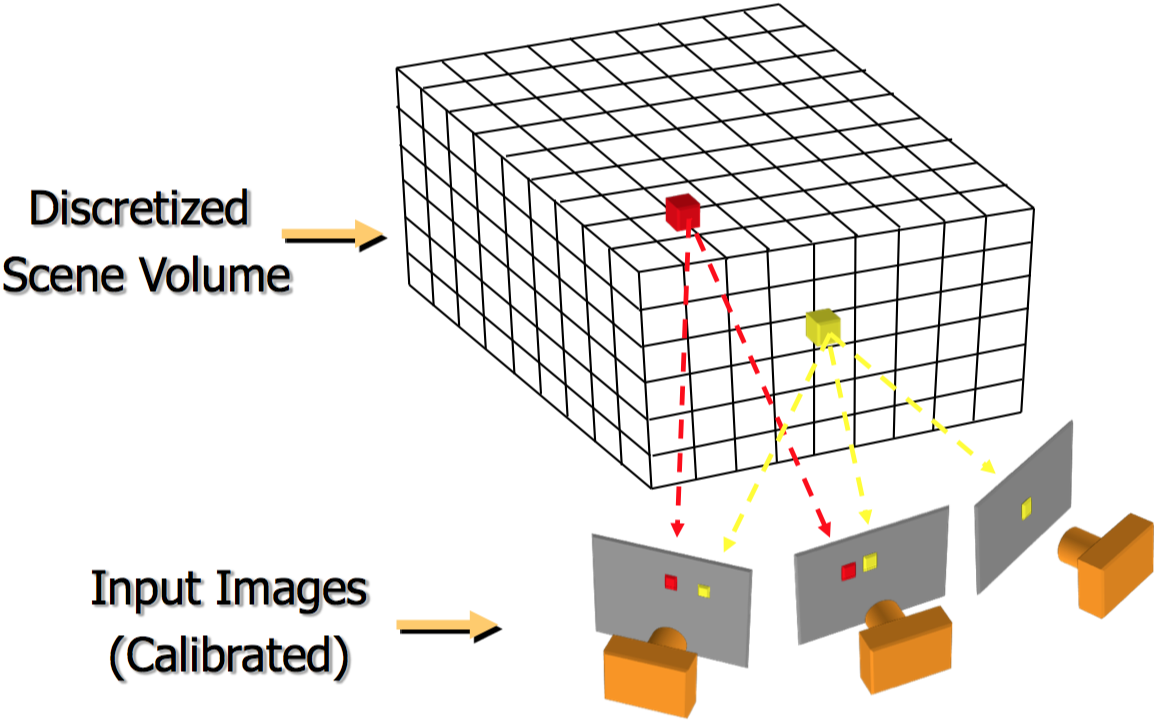
\includegraphics[width=0.8\textwidth]{taxo/volumetric_grid}
\caption{Voxel grid}
\end{figure}
Voxel grid can also be used for surface mesh extraction. Volemetric surface extraction accumulate information from depth maps, or laser scanned 3D points, and extracts a iso-surface using Marching Cube algorithm, or as a 3D binary(inside/outside) segmentation problem.

\subsection{Mesh}
One of the most popular surface mesh is triangular mesh.

\subsection{Normal map}
Normal map is typically visualized as a colour image, with each pixel colour coded as the normal. Each colour channel ranges from $[0, 255]$, and $n_x, n_y$ ranges from [-1, 1] while $n_z$ rangs from [0, 1]. The transformation between a normal and a colour is shown in Figure~\ref{fig:normal_map}.
\begin{align*}
n &= \frac{c}{128}-1\\
c &= 128\cdot(n+1)
\end{align*}

\begin{figure}[h]
\centering
\begin{tabular}{cc}
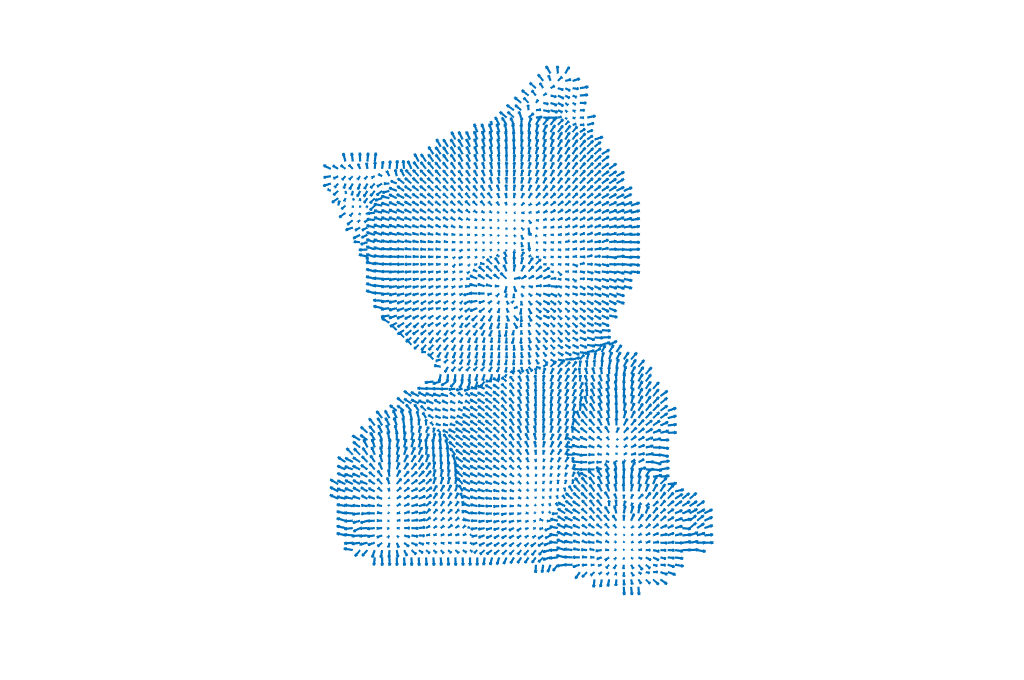
\includegraphics[width=0.5\textwidth]{taxo/normal_arrow}&
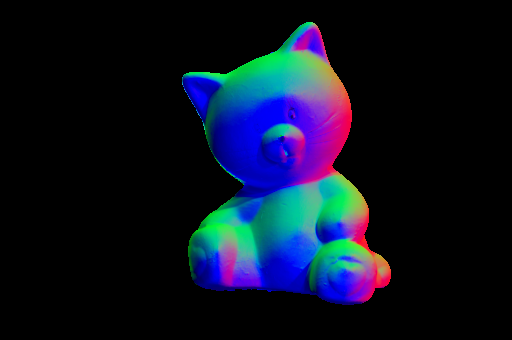
\includegraphics[width=0.5\textwidth]{taxo/normal_colour}\\
\end{tabular}
\caption{Representation of normal map}
\label{fig:normal_map}
\end{figure}

\section{Summary}
Our taxonomy focuses on the visual cues detected in images, which is utilized by various techniques. Conceptualize these visual cues as dimension of the 3D reconstruction problem, we have an abstraction which allow us to think of algorithms as volumes within a $n-$dimensional problem space. Existing algorithms can be introduced into this framework based on the main visual cue used for reconstruction. Instances where these algorithms have been reported as supporting other forms of variation have been outlined, providing an initial mapping of the space that is summarized below in Table~\ref{tab:algo_label}.
\begin{table}[h]
  \centering
  \begin{tabular}{l*{5}{c}}
  \hline
  \textbf{Technique} & Setup & Dom & Cue & Charact & Rep\\
  \hline
  PMVS & $C_n$ & $S$ & $T$ & $P$ & $P$\\
  Goesele & $C_n$ & $S$ & $T$ & $D$ & $D$\\
  Woodham & $C_1L_n$ & $T$ & $I$ & $LDS$ & $N$\\
  Hertzemann & $C_1L_n$ & $T$ & $I$ & $MDM$ & $N$\\
  Gray code & $C_1P$ & $T$ & $I$ & $B$ & $P$\\
  \hline
  \end{tabular}
  \label{tab:algo_label}
  \caption{Algorithm classification based on the new taxonomy}
\end{table}
